% small.tex
\documentclass[aspectratio=169]{beamer}
\usetheme{Boadilla}
\usepackage{amsmath}
\usepackage{graphicx}
\usepackage{wrapfig}
%algorithms and pseudo code
\usepackage{algorithm}
\usepackage[noend]{algpseudocode}
\usepackage{numprint}
\usepackage{subcaption}
\usepackage{media9}
\usepackage{bibentry}
\usepackage[autoplay,loop]{animate}
\usepackage[justification=centering]{caption}
\nobibliography*

\setbeamertemplate{bibliography item}[text]
\setbeamertemplate{author in head/foot}{\insertshortauthor}
\setbeamertemplate{navigation symbols}{}

\newcommand{\lenitem}[2][.6\linewidth]{\parbox[t]{#1}{\strut #2\strut}}
\newcommand{\outline}{
  \begin{frame}<beamer>
    \frametitle{Outline}
    \tableofcontents[currentsection]
  \end{frame}
}

\begin{document}

\title[Load Balancing on Many-Core and Accelerated Systems]{

Session 4: Heterogeneous Applications: Maximizing Benefits While Minimizing Cost

\textbf{Load Balancing on Many-Core and Accelerated Systems}
}

\author[C. Smith]{\underline{Cameron W. Smith}, Gerrett Diamond, and Mark S. Shephard}

\institute[SCOREC]{
Scientific Computation Research Center \\
Rensselaer Polytechnic Institute
}

\date{April 25, 2019}


%----------- titlepage ----------------------------------------------%
\begin{frame}[plain]
  \titlepage
\end{frame}

%----------------------------------------------------------------------%
%----------- Systems --------------------------------------------------%
%----------------------------------------------------------------------%
\begin{frame}
  \frametitle{Load Balancing, Performance, and Scalability}
  \begin{itemize}
  \item Load Balancing - distributing work to maximize performance on a
  given machine
  \item Performance - time to solution
  \item Scalability - efficiency with increase in computing power
    \begin{itemize}
    \item Weak - increase problem size with increase in computing power
    \item Strong - fixed problem size as computing power increases
    \end{itemize}
  \item High performance procedures are not necessarily
    scalable or portable
  \item Scalable procedures are not necessarily portable
  \end{itemize}
\end{frame}

\section{Manycore and Accelerated Systems}
\begin{frame}
  \frametitle{Manycore and Accelerated Systems}
  Manycore
  \begin{itemize}
    \item processor with many homogenous cores
    \item some reserved cores and hardware threads to handle OS iteractions
    \item all cores can communicate with other cores
    \item possibly multiple NUMA domains
  \end{itemize}
  Accelerated
  \begin{itemize}
    \item Host processor - dispatches accelerator work, facilitates
      communications, OS iteractions
    \item Accelerator - does 90\% of the work
  \end{itemize}
\end{frame}

%----------------------------------------------------------------------%
%----------- Section --------------------------------------------------%
%----------------------------------------------------------------------%
\section{Partitioning and Load Balancing}
\begin{frame}
  \frametitle{Motivation and Focus}
  \begin{columns}
    \begin{column}{0.7\textwidth}
      Many evolving distributed simulations have: \\
      \begin{itemize}
        \item Complex relational structures.
        \item Irregular forms of computational and communication costs.
        \item Evolving imbalance of work. %Define Imbalance
        \item Multiple criteria that need balancing simultaneously.
      \end{itemize}
      Applications
      \begin{itemize}
        \item Libraries composed into a single executable
        \item Bulk synchronus parallel execution \\
          {\small \texttt (1) work (2) communicate (3) goto 1}
        \item Global runtime systems are a different beast... some of this may apply.
      \end{itemize}
    \end{column}
    \begin{column}{0.3\textwidth}
      \begin{figure}
        \centering
        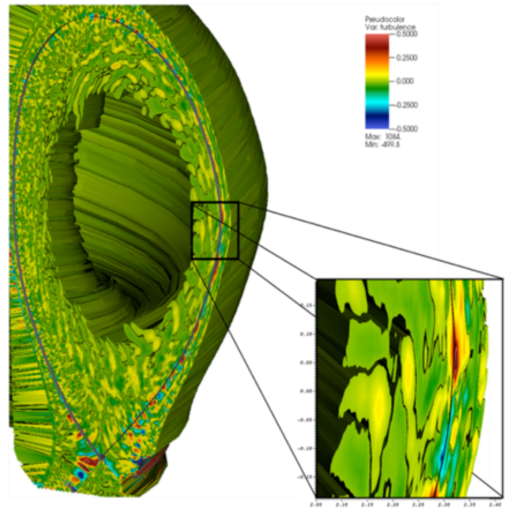
\includegraphics[width=.75\textwidth]{figures/xgcCase.png} \\
        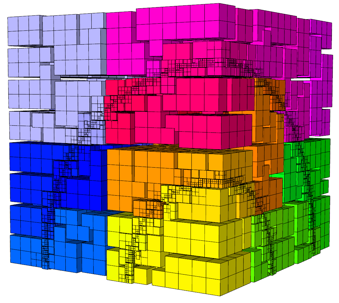
\includegraphics[width=.75\textwidth]{figures/laghos_sedov.png}\\
        \tiny{XGC fusion plasma physics (top) and MFEM Laghos Sedov blast
        (bottom)}
      \end{figure}
    \end{column}
  \end{columns}
\end{frame}

\begin{frame}
  \frametitle{Common Methods for Partitioning}
  \begin{columns}
    \begin{column}{0.4\textwidth}
      \begin{itemize}
        \item Multilevel Graph Methods %Discuss poor scaling
          \begin{itemize}
            \item ParMETIS
            \item Zoltan
          \end{itemize}
        \item Geometric Methods %Require coordinates
          \begin{itemize}
            \item Recursive Coordinate Bisection (RCB)
            \item Recursive Inertial Bisection (RIB)
            \item Multi-Jagged
          \end{itemize}
        \item Diffusive Methods %Improve a partition efficiently
          \begin{itemize}
            \item Label Propagation
            \item ParMA and EnGPar
          \end{itemize}
      \end{itemize}
    \end{column}
    \begin{column}{0.6\textwidth}
      \begin{figure}
        \centering
        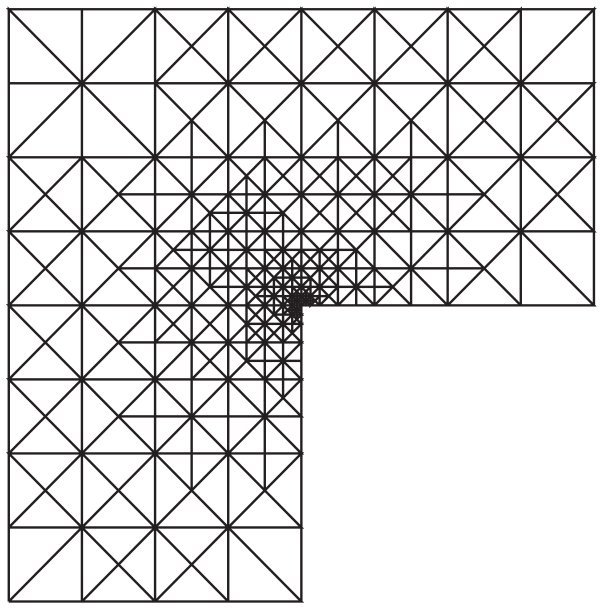
\includegraphics[width=.32\textwidth]{figures/mitchellMesh.png}
        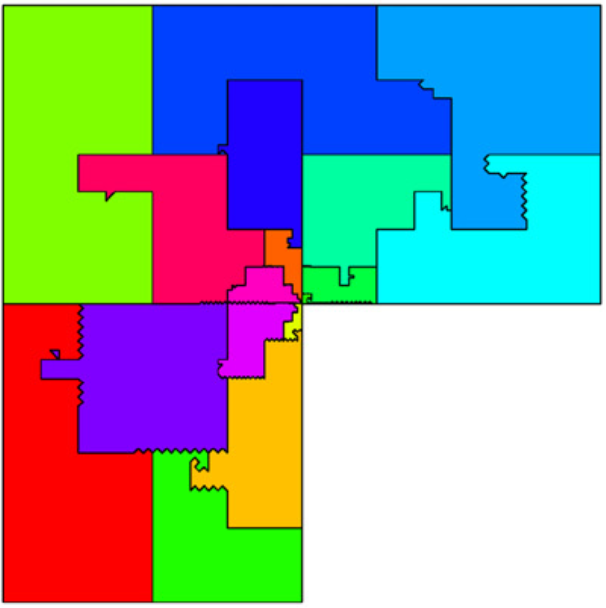
\includegraphics[width=.32\textwidth]{figures/mitchellHSFC.png}
        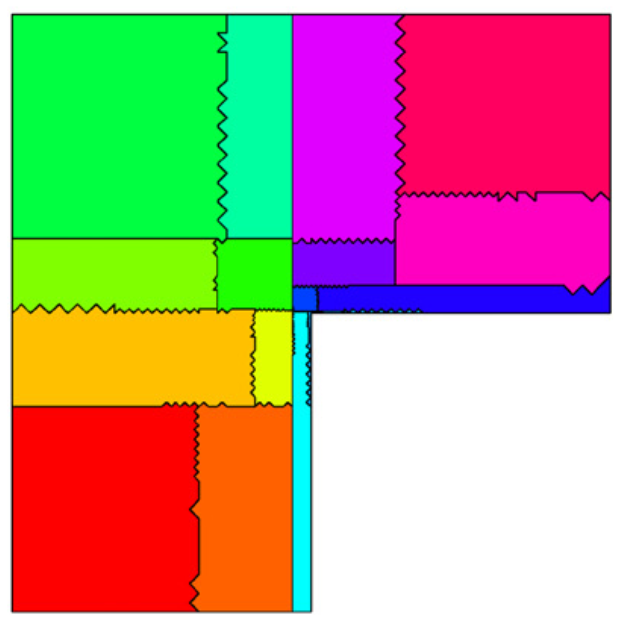
\includegraphics[width=.32\textwidth]{figures/mitchellRCB.png} \\
        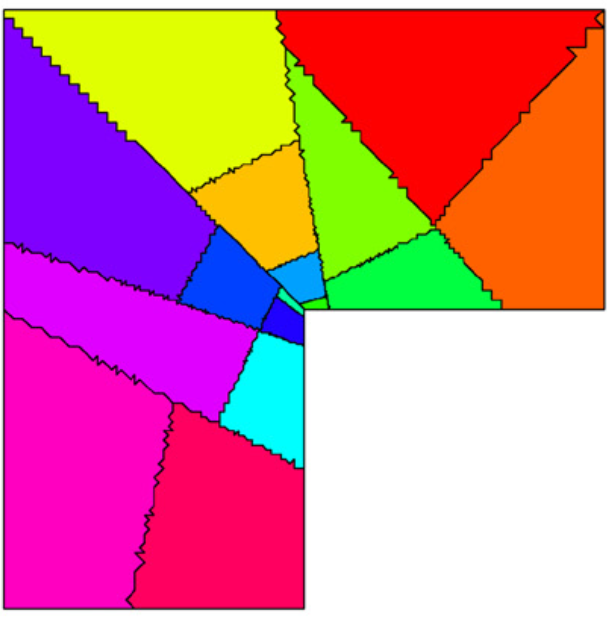
\includegraphics[width=.32\textwidth]{figures/mitchellRIB.png}
        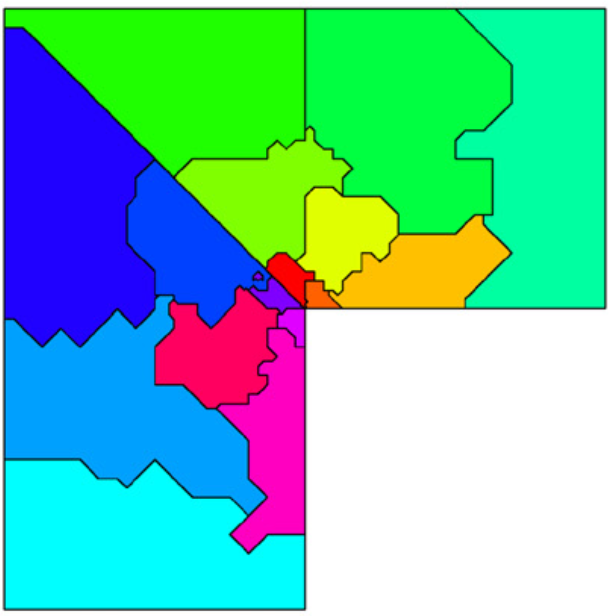
\includegraphics[width=.32\textwidth]{figures/mitchellParmetis.png} \\
        \small{Top to bottom, left to right: mesh, space filling curve,
        coordinate bisection, inertial bisection, multi-level k-way.} \\
        \tiny{``A refinement-tree based partitioning method for dynamic load
        balancing with adaptively refined grids'', William F. Mitchell}
      \end{figure}
    \end{column}
  \end{columns}
\end{frame}

\section{EnGPar - a graph based diffusive load balancer}

\begin{frame}
  \frametitle{What is EnGPar?}
  \begin{itemize}
  \item A partitioning tool to complement existing multi-level and geometric methods.
  \item Provides a diffusive load balancing algorithm for partition improvement and supports multi-criteria partitioning.
  \item Utilizes a specialized multigraph structure to represent relation based data.
  \item Implemented to support efficient data parallel operations on accelerators and vector units in many core processors.
  \end{itemize}
\end{frame}

\begin{frame}
  \frametitle{Mapping application data to EnGPar}
  %Before using EnGPar a simulation must first map its data to the N-graph
  To map to EnGPar, applications must:
  \begin{itemize}
  \item Define units of work as the graph vertices.
  \item Decide on the mode (regular vs. hyper) of edges to use.
  \item Create (hyper)edges between the vertices whose corresponding work relate to each other.
  \end{itemize}
\end{frame}


\begin{frame}
  \frametitle{Diffusive Partitioning}
  \begin{algorithm}[H]
    \caption{Diffusive Load Balancing Framework}
    \label{alg:engpar}
    \small
    \begin{algorithmic}[1]
      \Procedure{Balance}{$ngraph$,$entity\_types$}
      \ForAll{$t \in entity\_types$}
      \While{imbalance of $t >$ tolerance}
      \Call{RunStep}{$ngraph$,$t$}
      \If{Balancing Stagnates}
      \State break
      \EndIf
      \EndWhile
      \EndFor
      \EndProcedure

      \Procedure{RunStep}{$ngraph$,$t$}
      \State $sides = makeSides(ngraph)$
      \State $weights = makeWeights(ngraph,sides,t)$
      \State $targets = makeTargets(ngraph,sides,weights)$
      \State $queue = makeQueue(ngraph)$
      \State $plan = select(ngraph,targets,queue)$
      \State $ngraph.migrate(plan)$
      \EndProcedure
    \end{algorithmic}
  \end{algorithm}
\end{frame}

\begin{frame}
  \frametitle{Queue}
  \begin{figure}
    \centering
    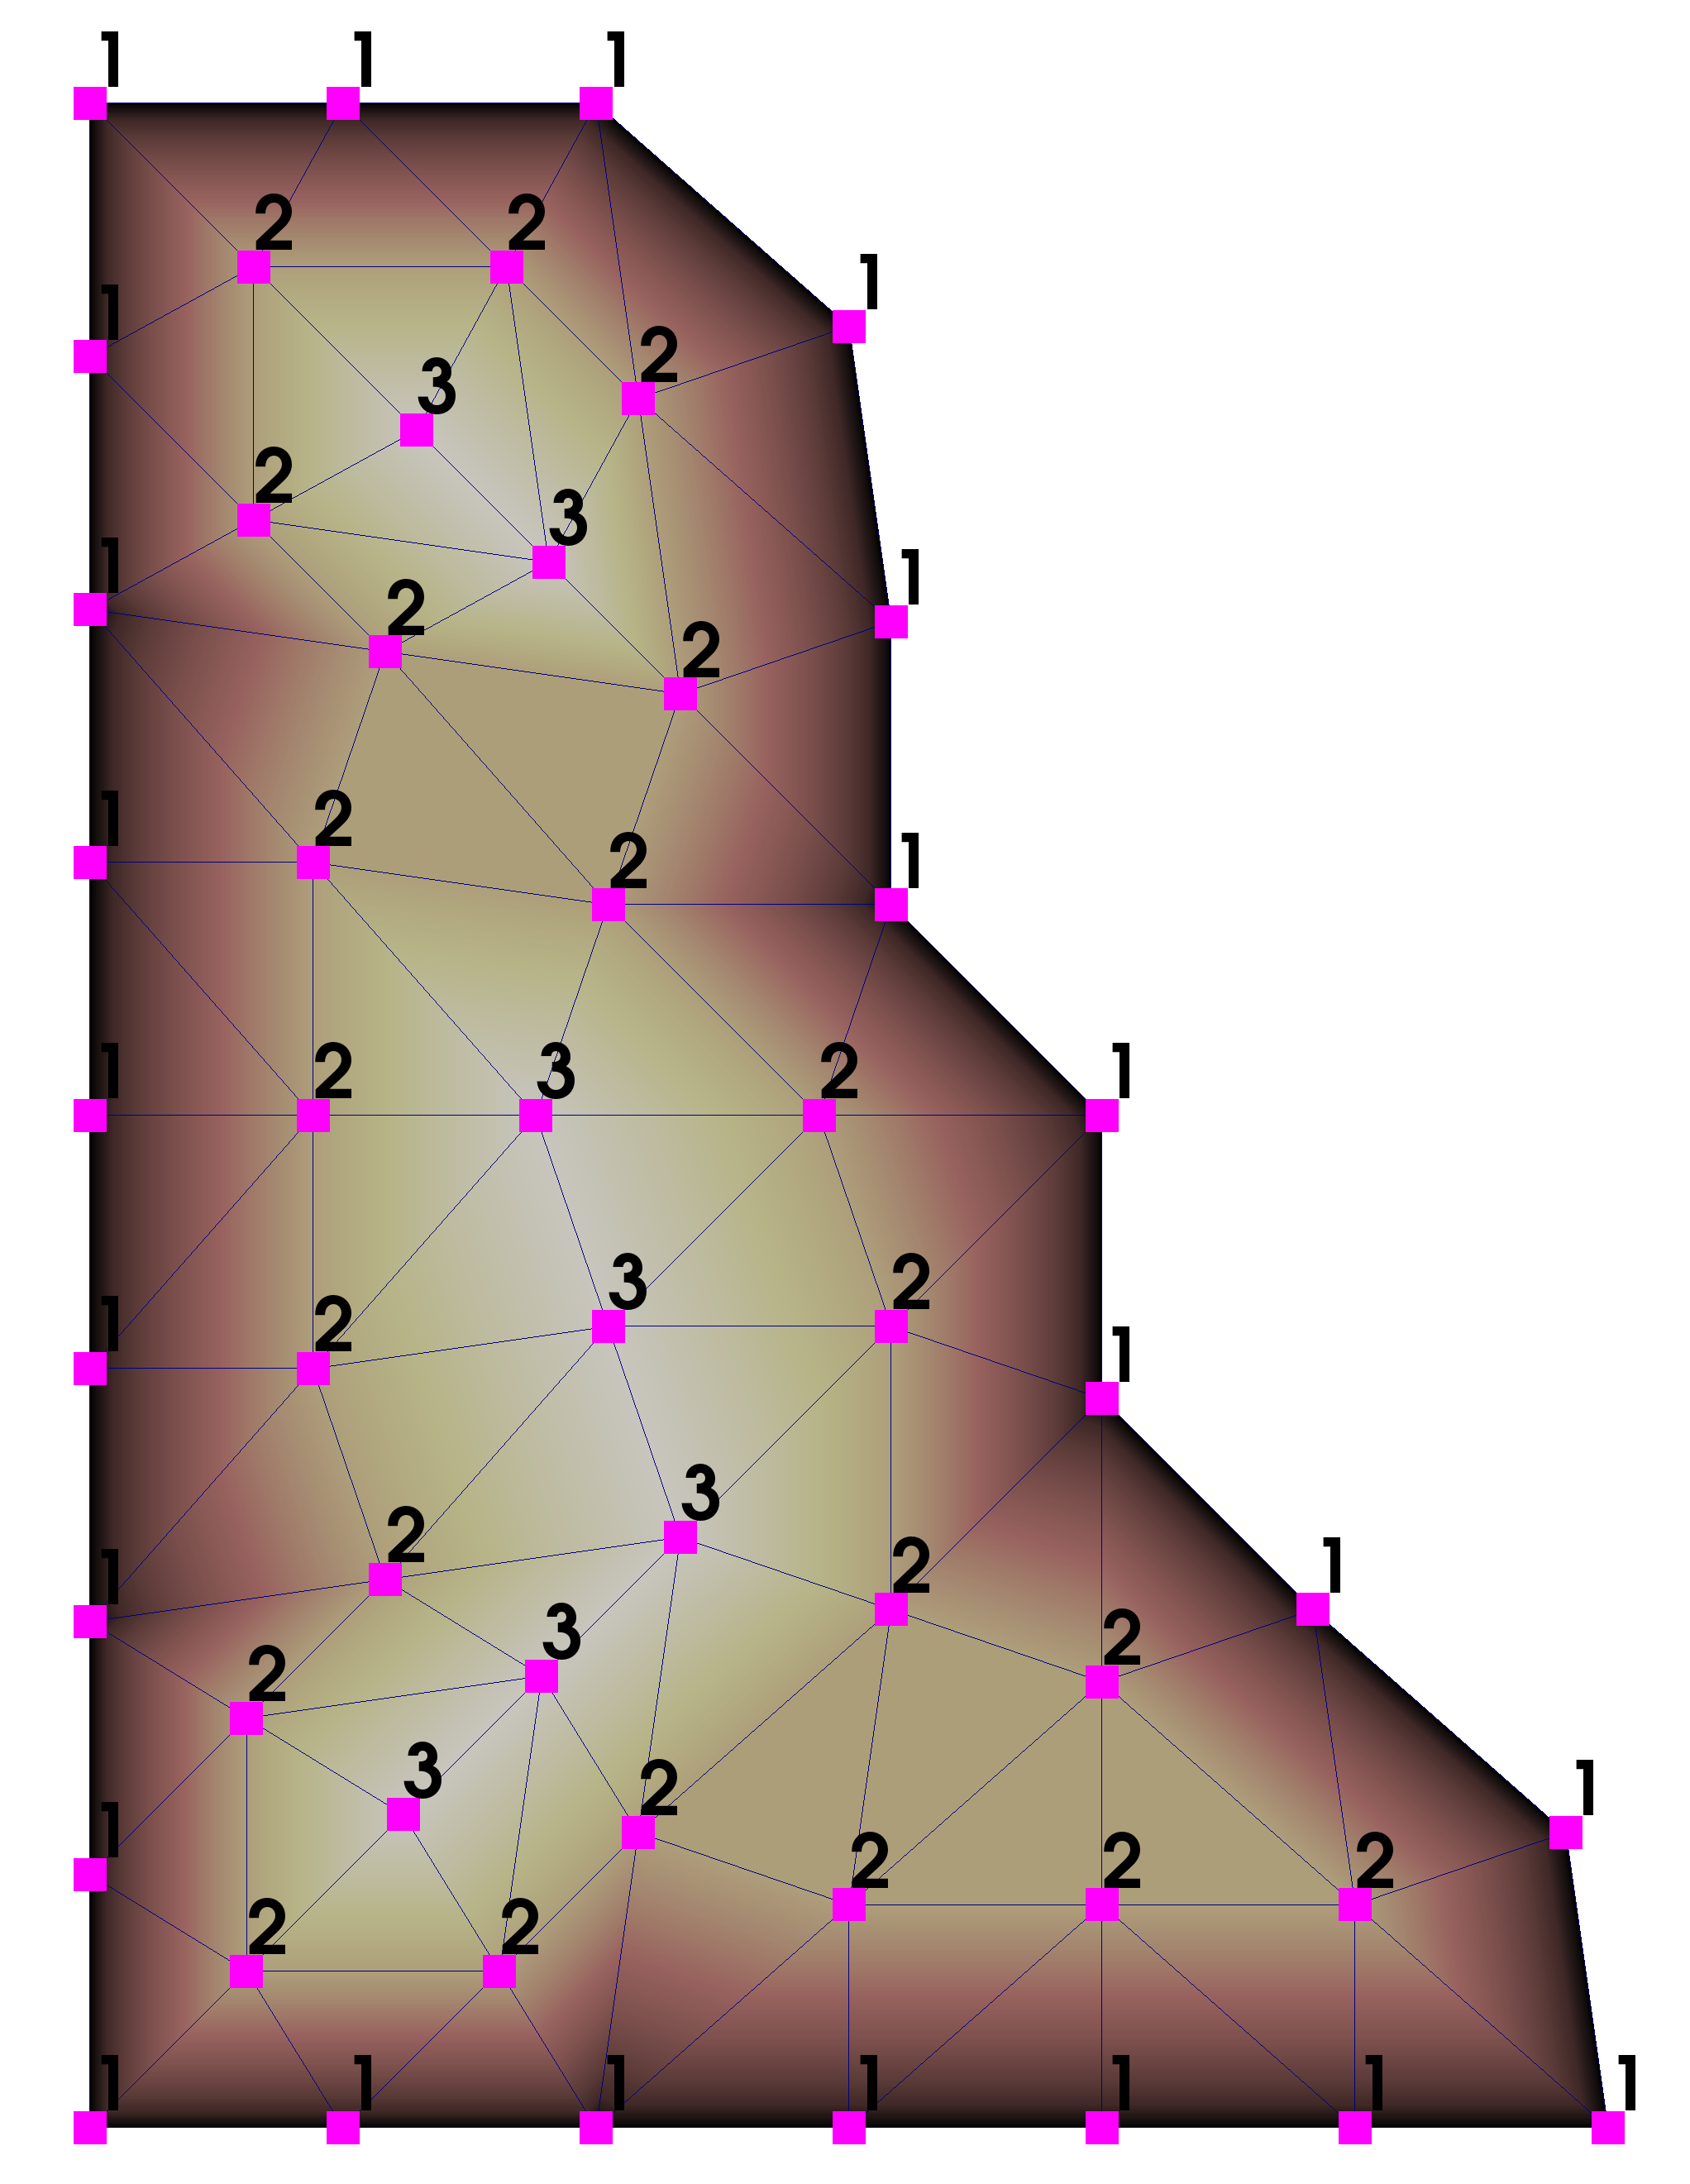
\includegraphics[width=.3\textwidth]{../accelerated_cse19/figures/2dTreeDepth.png}
    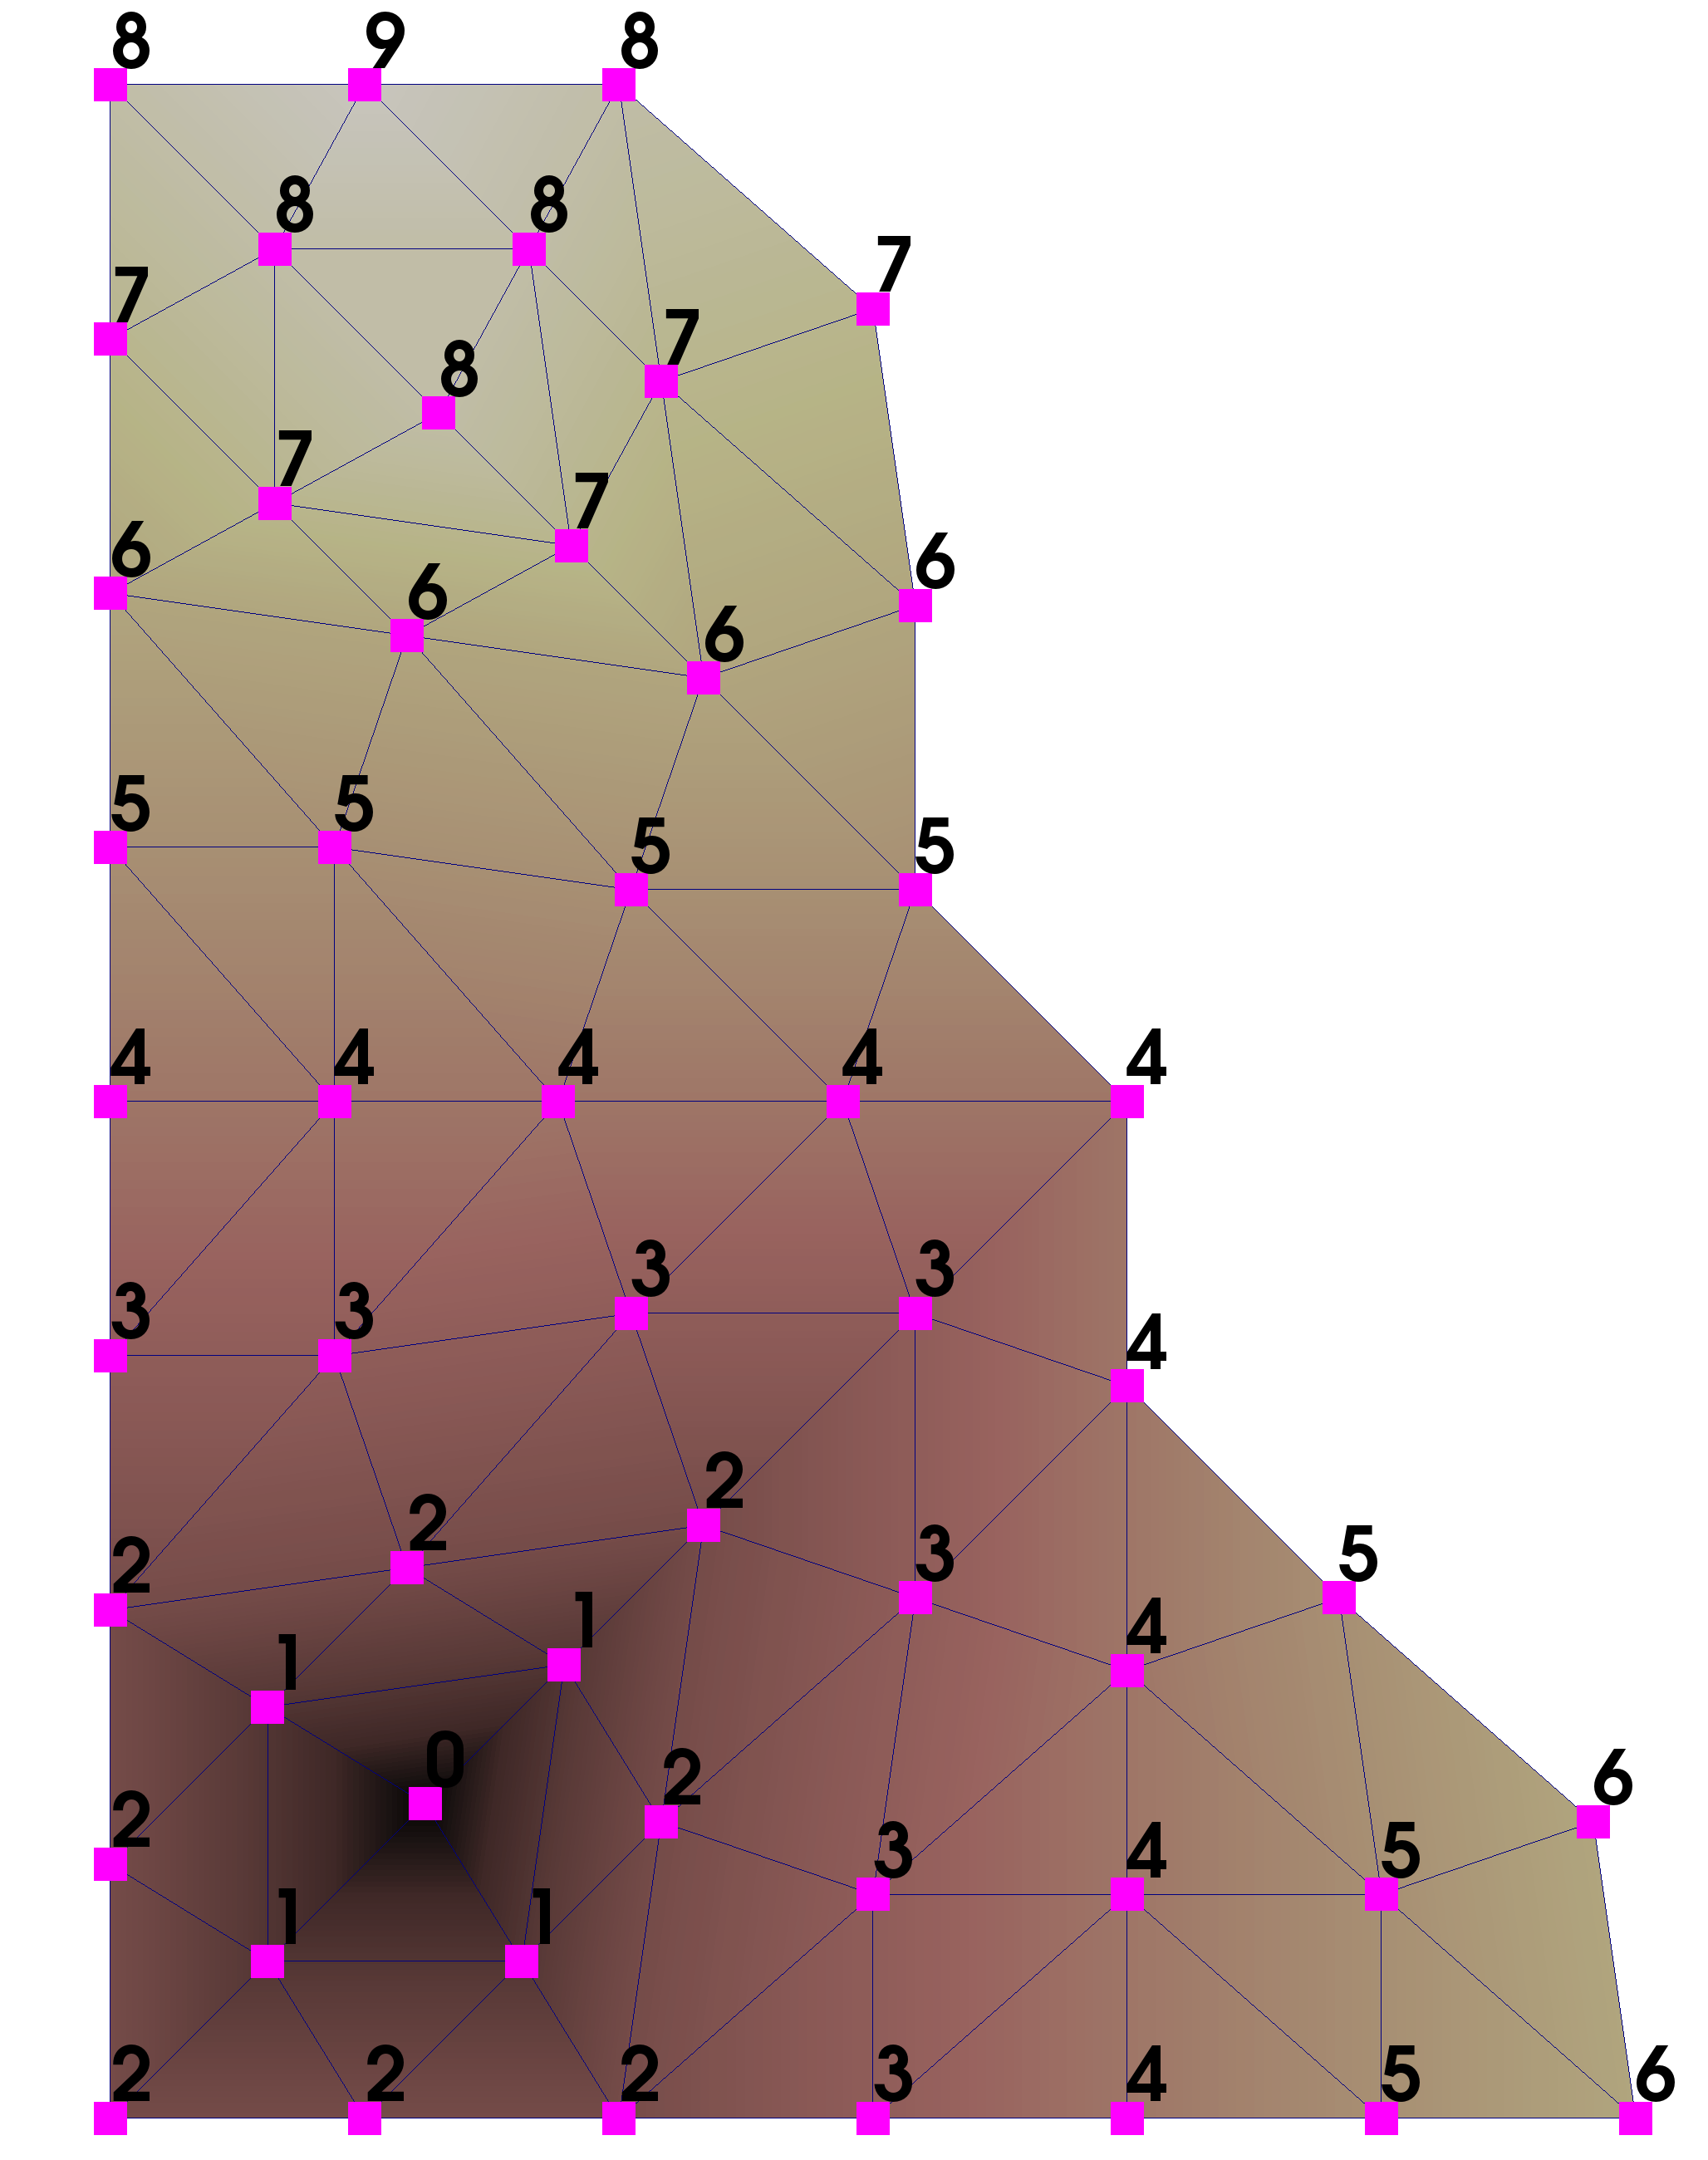
\includegraphics[width=.31\textwidth]{../accelerated_cse19/figures/2dDistance.png}
  \end{figure}
      (left) The distance from each vertex to the boundary and (right) the
    distance from the core vertex (marked with a zero near the
    bottom left corner).
\end{frame}

\section{Partition Improvement Results}
\begin{frame}
  \frametitle{}
  \center \huge{Partition Improvement Results}
\end{frame}

\begin{frame}
  \frametitle{Problem Setup}
  We evaluate EnGPar's ability to improve vertex-centric
  and element-centric partitions created by ParMETIS.\\
  \medskip
  EnGPar is set to balance a mesh for a finite element and finite volume analysis where:
  \begin{itemize}
    \item Scalability of matrix formation is sensitive to secondary entity imbalance.
    \item Linear algebra routines are sensitive to the imbalance of degrees of freedom.
    \item Degrees of freedom are associated with primary entities.
  \end{itemize}
  \bigskip
  EnGPar first balances the DOF holders and then the secondary entity.
  target imbalance of 1.05. \\
  The imbalance of a given type (vtx, edge, face, or region) is defined as the 
  max part weight divided by the avg part weight.
\end{frame}

\begin{frame}
  \frametitle{Element Partition: Problem Setup}
  \medskip
  Element-centric tests were run on a billion element mesh. \\
  All experiments were run on the Mira BlueGene/Q system with one process per
  hardware thread. \\
  \smallskip
  Initial partitions are built using:
  \begin{itemize}
  \item Global ParMETIS part k-way to 8Ki($8*2^{10}$) parts.
  \item Local ParMETIS part k-way from 8Ki to 128Ki, 256Ki, and 512Ki parts.
  \end{itemize}
  The partitions before using EnGPar:\\
  \begin{table}[!h]
    \centering
    \begin{tabular}{||c|c|c|c||}
      \hline
      Number of Parts &128Ki&256Ki&512Ki \\
      \hline
      Elements per part & 9,836 & 4,918&2,459  \\
      \hline
      Vertex imbalance & 1.13 & 1.18 & 1.53 \\
      \hline
      Element imbalance & 1.02& 1.02& 1.02\\
      \hline
    \end{tabular}
  \end{table}
\end{frame}

\begin{frame}
  \frametitle{Element Partition: Mesh Vertex and Element Imbalance}
  \begin{figure}
    \centering
    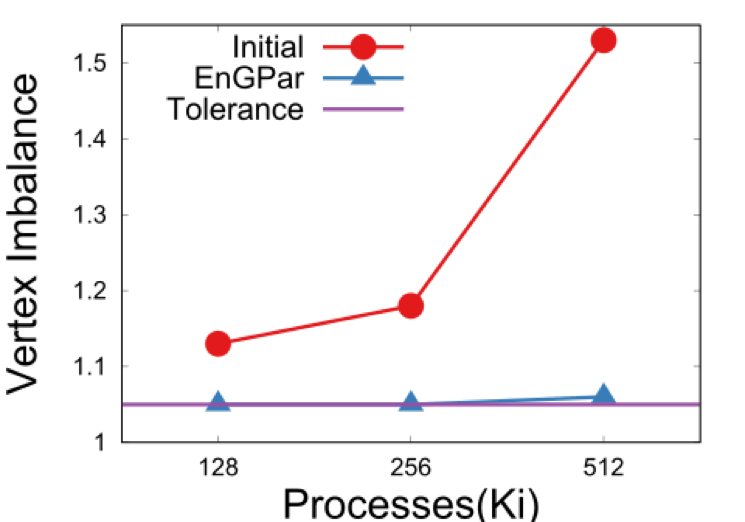
\includegraphics[width=.49\textwidth]{../accelerated_cse19/figures/elmPtn_vtxImb.png}
    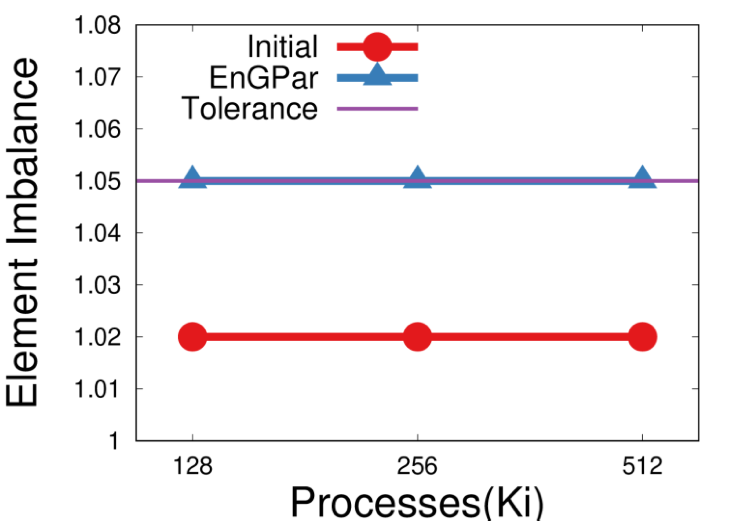
\includegraphics[width=.49\textwidth]{../accelerated_cse19/figures/elmPtn_elmImb.png} \\
    Mesh vertex imbalances is reduced from 13\% to 5\% for 128Ki, 18\% to 5\% for
    256Ki, and 53\% to 6\% for 512Ki.  Edge cut is increased by 1\%.
  \end{figure}  
\end{frame}

\begin{frame}
  \frametitle{Vertex Partition: Problem Setup}
  \medskip
  Vertex-centric tests were run on a 60 million element mesh. \\
  All experiments were run on the Mira BlueGene/Q system. \\
  \smallskip
  Initial partitions are built using:
  \begin{itemize}
  \item Global ParMETIS part k-way to 8Ki($8*2^{10}$) parts.
  \end{itemize}
  The partitions before using EnGPar: \\
  \begin{table}[!h]
    \centering
    \begin{tabular}{||c|c|c|c|c||}
      \hline
      Number of Parts   & 1Ki   & 2Ki   & 4Ki   & 8Ki \\
      \hline
      Vertices per part & 17,984 & 8,992 & 4,496 & 2,248 \\
      \hline
      Vertex imbalance  & 1.05  & 1.05  & 1.05  & 1.05 \\
      \hline
      Element imbalance & 1.99  & 2.0  & 1.99  & 2.00 \\
      \hline
    \end{tabular}
  \end{table}
  ParMETIS sacrifices element imbalance for a low edge cut.
\end{frame}

\begin{frame}
  \frametitle{Vertex Partition: Mesh Element Imbalance and Edge Cut}
  \begin{figure}
    \centering
    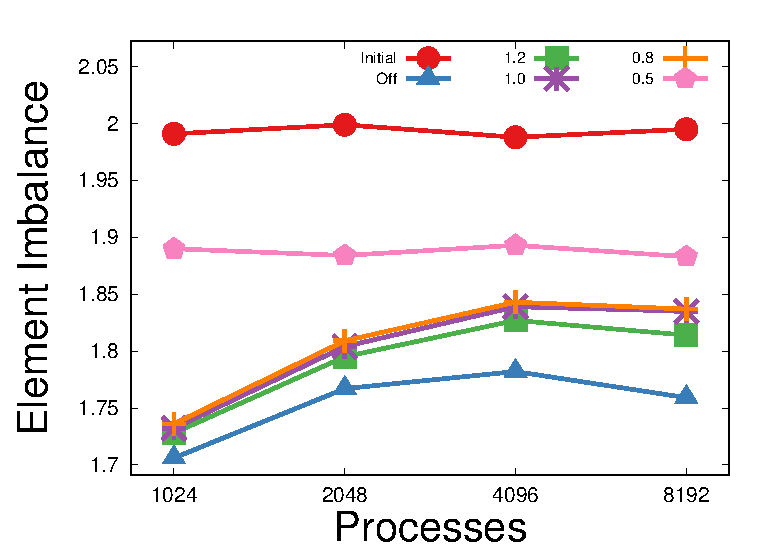
\includegraphics[width=.48\textwidth]{../accelerated_cse19/figures/eimb_v_cores.eps}
    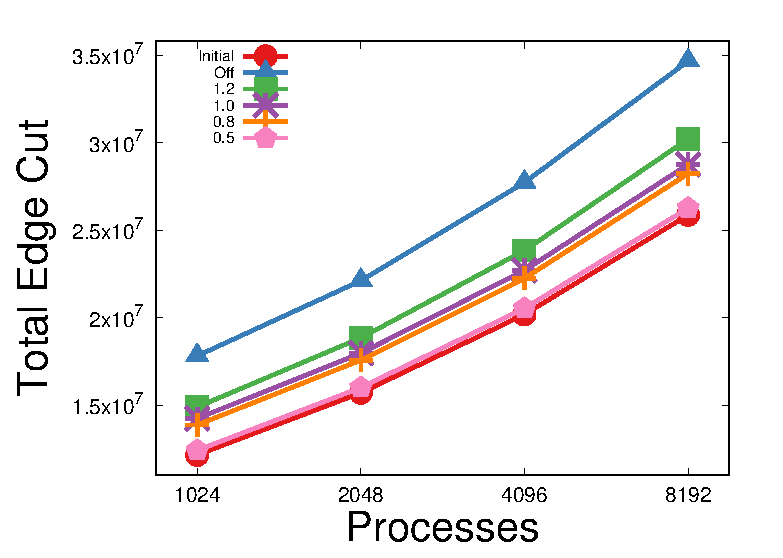
\includegraphics[width=.48\textwidth]{../accelerated_cse19/figures/ecut_v_cores.eps}\\
    Tuning the edge cut metric maintains the ParMETIS edge cut while reducing the
    edge imbalance by up to 5\%.
  \end{figure}  
\end{frame}

\section{Load Balancing On Accelerated Systems}

\begin{frame}
  \frametitle{}
  \center \huge{Load Balancing On Accelerated Systems}
\end{frame}

\begin{frame}
  \frametitle{Summit Computing Hardware}
  \textbf{Focus on GPUs; they provide 95\% of memory bandwidth and 98\% of FLOPs}
  \begin{itemize}
    \item 6 V100 and 2 P9 per node
    \item 4,608 nodes $\rightarrow$ 27,648 V100 and 9,216 P9
  \end{itemize}
  {
  \begin{table}[]
    \begin{tabular}{lrr}
      Processor   & Double Precision & Memory           \\
                  & TeraFLOPs        & Bandwidth (GB/s) \\
      V100        & 7.5              & 900              \\
      P9          & 0.5              & 135       \\
      P9/V100     & 7\%              & 15\% \\
      \\
      Full System &                  & \\
      V100        & 207,360          & 24,833,200       \\
      P9          & 4,608            & 1,244,160       \\
      P9/V100     & 2\%              & 5\%
    \end{tabular}
  \end{table}
  }
  % Summit GPUs: 207PF, 24 PB/s
  % Summit P9s:  4.6PF, 1 PB/s
  %from sc18-tutorial-pleiter.pdf
\end{frame}

\begin{frame}
  \frametitle{Summit Communication Hardware}
  205:1 ratio of aggregate node memory bandwidth to inter-node network bandwidth
    \begin{columns}
      \begin{column}{0.3\textwidth}
        \begin{figure}
          \centering
          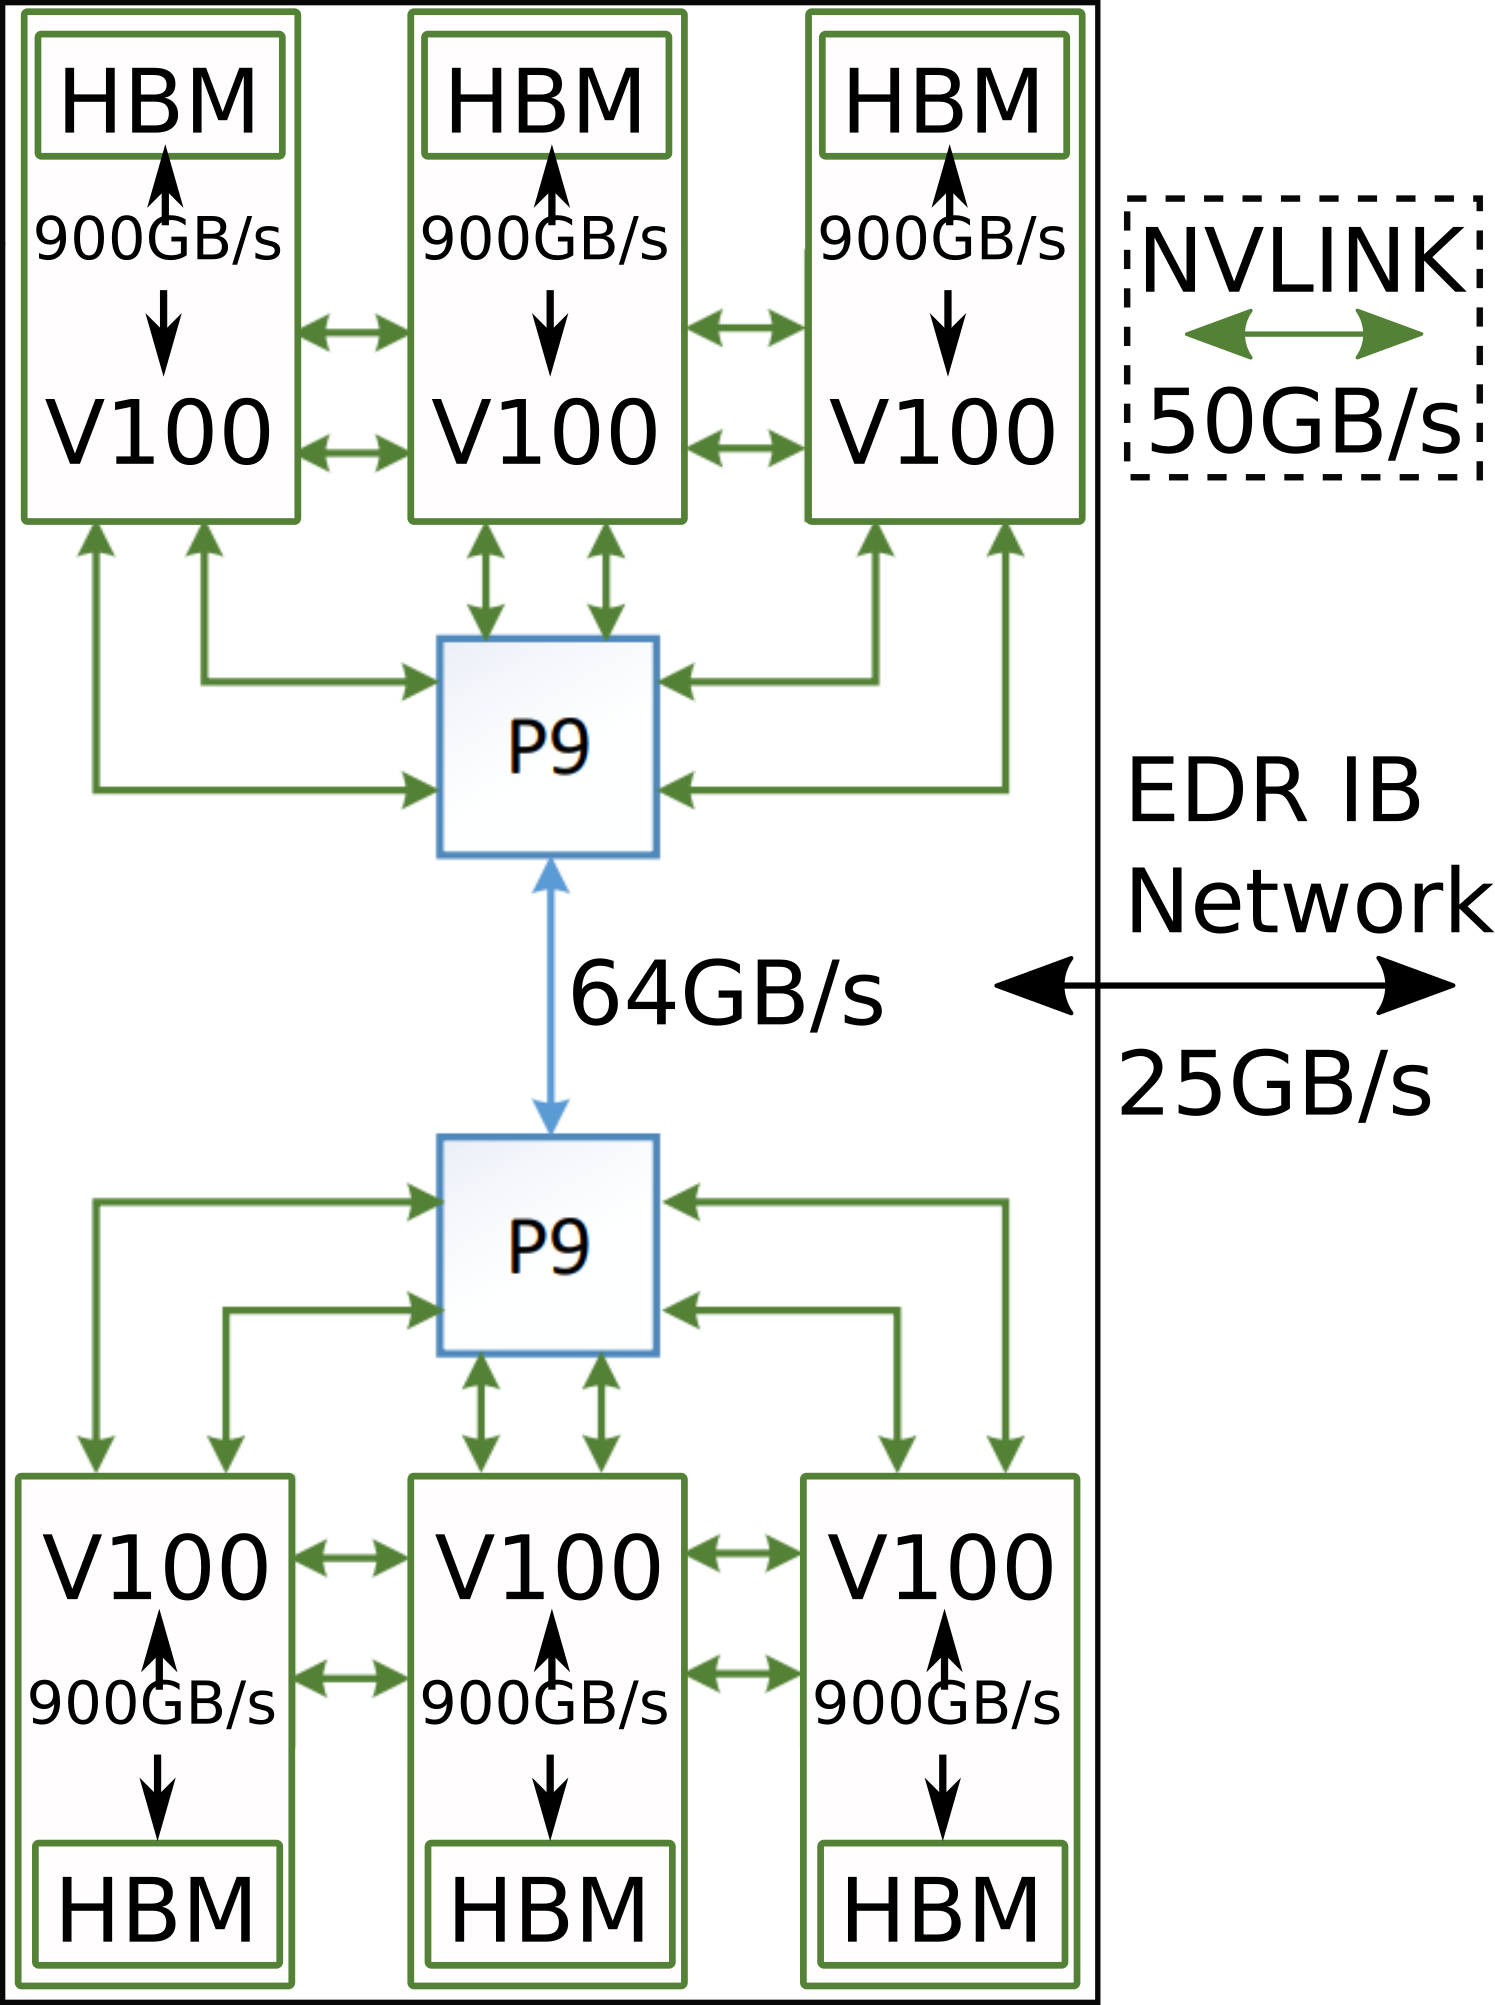
\includegraphics[width=.9\textwidth]{figures/summit-node.png}\\
          \tiny{J.Choquette. Hot Chips 2017. \\"Volta: Programmability and Performance"}
        \end{figure}
      \end{column}
    \begin{column}{0.7\textwidth}
      { \small
      \begin{table}[]
        \begin{tabular}{lrrr}
          System              & Stream       & Network     & Stream/ \\
                              & Triad (GB/s) & Peak (GB/s) & Network \\
          Summit (inter-node) & 5,130         & 25          & 205     \\
          Summit (intra-node) & 855          & 50          & 17      \\
          Stampede2           & 194          & 12          & 17      \\
          Mira                & 27           & 20          & 1.4
        \end{tabular}
      \end{table}
      }
    \end{column}
  \end{columns}
  %V100 stream triad from Jack Choquette HotChips 2017 presentation "Volta: Programmability and Performance"
  %Mira network ref: PAMI: A Parallel Active Message Interface for the Blue Gene/Q Supercomputer
  %Mira stream triad ref: Bob Walkup "Application Performance Characterization and Analysis on Blue Gene/Q"
  %On a Skylake cluster like Stampede2 the ratio is in the range of 250:1 (~3 TFDP for two socket
  % skylake https://colfaxresearch.com/xeon-2017/ and 
  % 12GB/s Omnipath https://portal.tacc.utexas.edu/user-guides/stampede2#overview-network)
  % SKX stream triad: "TACC Technical Report TR-17-01 Benchmarking the Intel Xeon Platinum 8160 Processor"
\end{frame}

\begin{frame}
  \frametitle{FUN3D - Finite Volume CFD}
  Eric Nielsen and Aaron Walden at NASA Langley \\
  Summit ESP: ``Enabling Human Exploration of the Red Planet''
  \begin{columns}
    \begin{column}{0.5\textwidth}
      Goals
      \begin{itemize}
        \item Science: Better understanding of retropropulsion flow physics during Mars entry of human-scale lander
        \item Computational: Demonstrate production readiness and efficiency advantages of GPU implementation at scale
      \end{itemize}
    \end{column}
    \begin{column}{0.5\textwidth}
      \begin{figure}
        \centering
        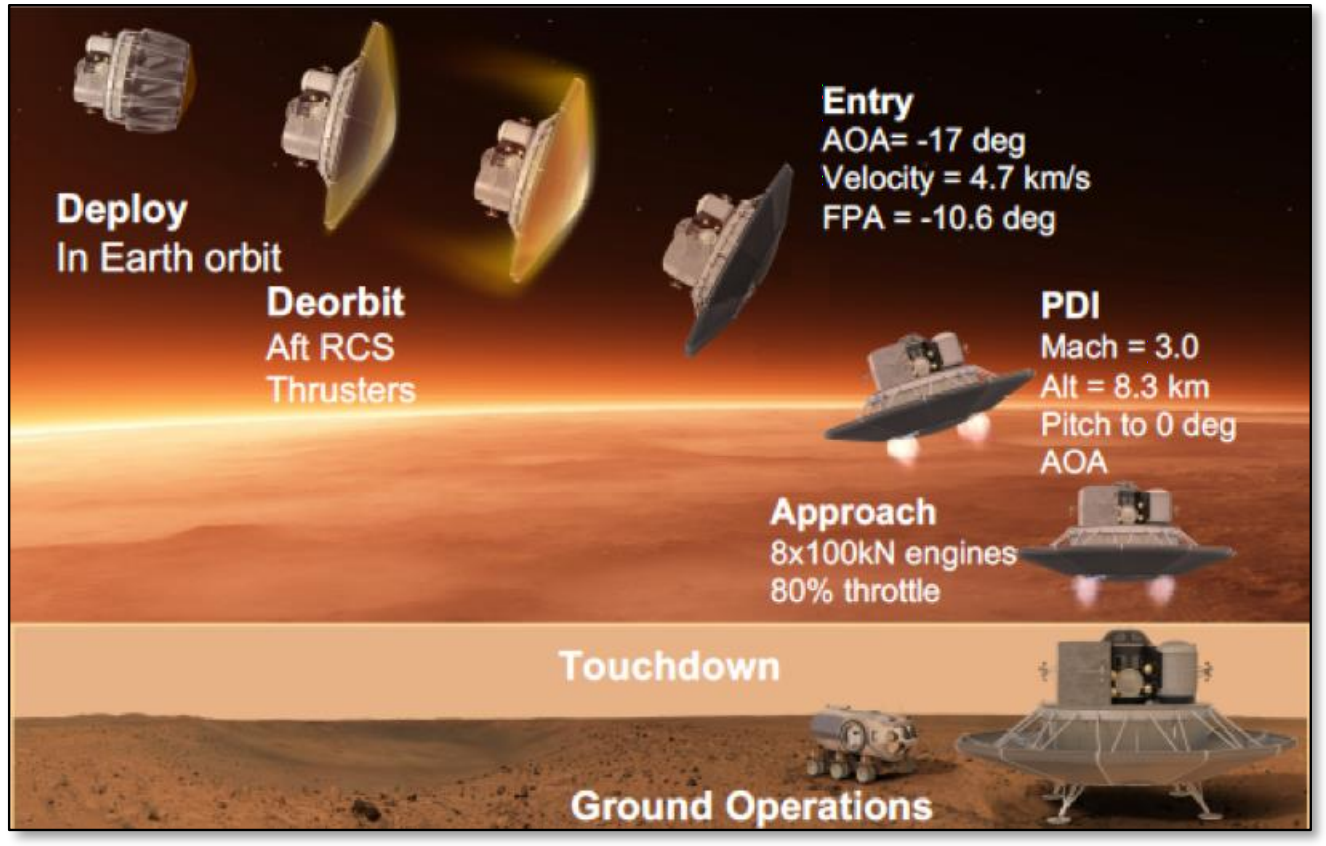
\includegraphics[width=.9\textwidth]{figures/fun3d-EDL.png}
      \end{figure}
    \end{column}
  \end{columns}
\end{frame}

\begin{frame}
  \frametitle{FUN3D - Early Summit Results (E. Nielsen and A. Walden)}
  \begin{columns}
    \begin{column}{0.5\textwidth}
      Partitioning Approach
      \begin{itemize}
        \item ParMETIS: mesh vertices $\rightarrow$ graph nodes, 
          mesh edges $\rightarrow$ graph edges
        \item Mesh vertices hold DOFs
        \item EnGPar is integrated and being tested
      \end{itemize}
      Weak Scaling - nearly linear
      \begin{itemize}
        \item 12.8M vertices per node. 13.2B vertices (58B elements) at 1024
          nodes.
        \item GPU: MPI+CUDA, 3 ranks/socket, MPI via GPUDirect
        \item CPU: MPI+OpenMP, ranks/socket, 168 threads per node (SMT4)
      \end{itemize}
      GPU node-level performance is 23x-37x faster at scale than CPUs
    \end{column}
    \begin{column}{0.5\textwidth}
      \begin{figure}
        \centering
        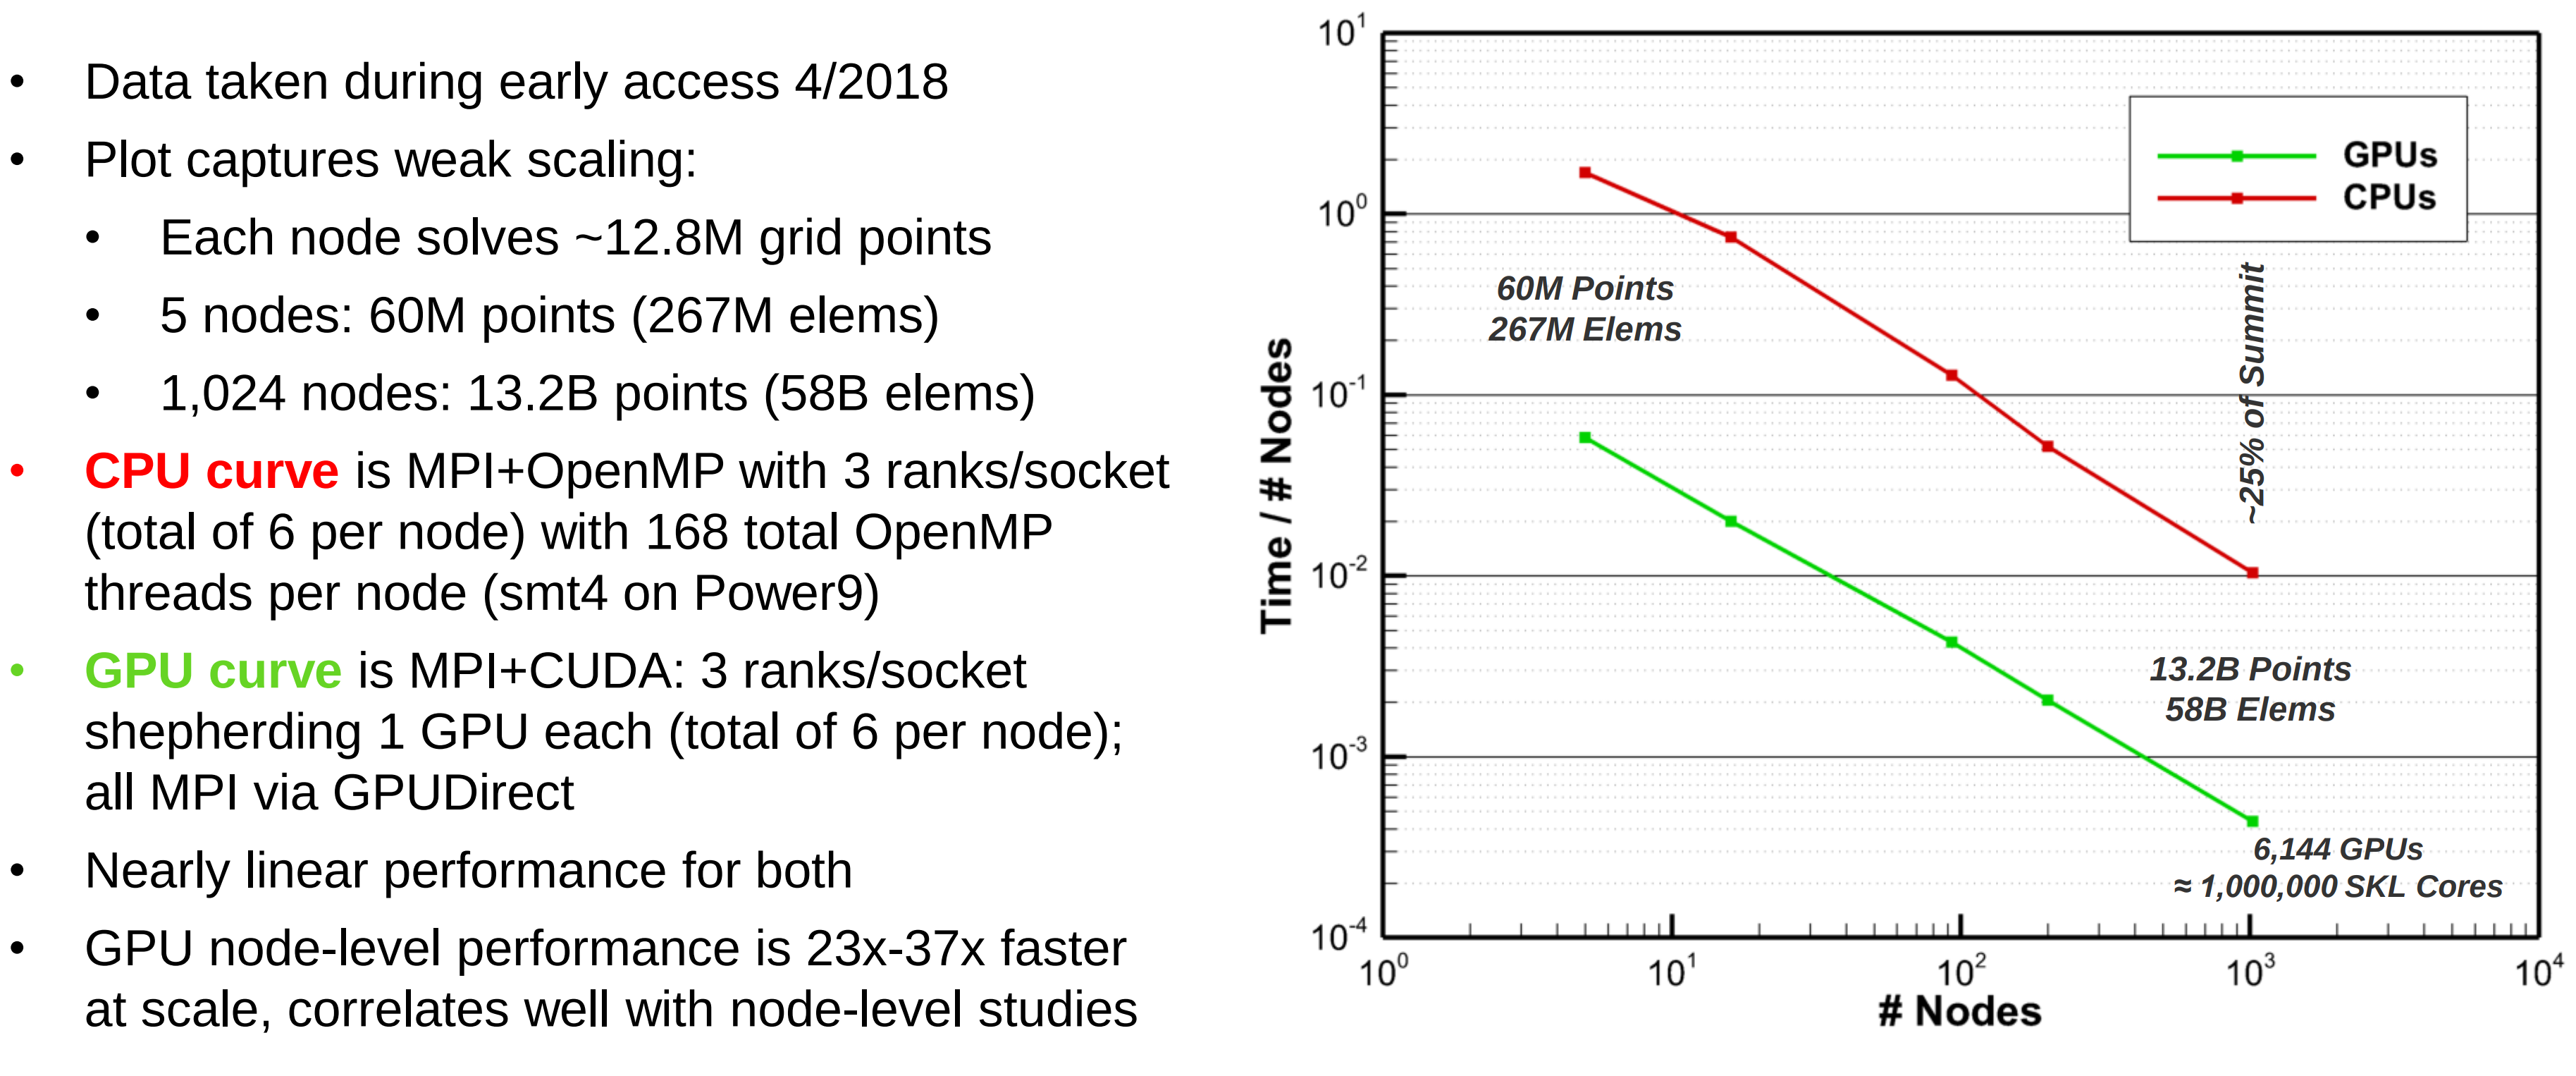
\includegraphics[width=\textwidth]{figures/fun3d-summit.png}
      \end{figure}
    \end{column}
  \end{columns}
\end{frame}

\begin{frame}
  \frametitle{XGC - Fusion Plasma Physics}
  CS Chang, Princeton Plasma Physics Laboratory \\
  Summit ESP: ``Using XGC to predict ITER’s boundary plasma performance and its impact on fusion efficiency''
  \begin{columns}
    \begin{column}{0.5\textwidth}
      Goals
      \begin{itemize}
        \item Science: Study tokamak plasma performance near boundary
	\item Computational: Develop platform for multiscale plasma physics simulations on leadership systems
      \end{itemize}
    \end{column}
    \begin{column}{0.5\textwidth}
      \begin{figure}
        \centering
        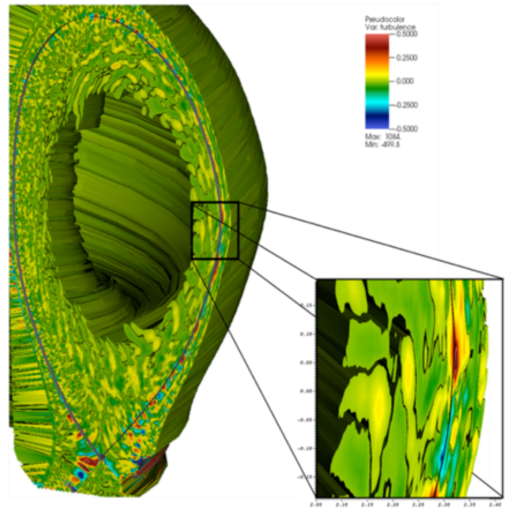
\includegraphics[width=.7\textwidth]{figures/xgcCase.png} \\
        \tiny{DIII-D Geometry: Boundary turbulence saturates 
        in $<$ 0.1ms, core turbulence in a few ms.}
      \end{figure}
    \end{column}
  \end{columns}
\end{frame}

\begin{frame}
  \frametitle{XGC - Partitioning Approach (CS Chang)}
  \begin{columns}
    \begin{column}{0.5\textwidth}
      %https://scorec.rpi.edu/~shephard/some%20fusion%20stuff/xgc-book-chapter.pdf
      %https://cug.org/proceedings/cug2016_proceedings/includes/files/pap178s2-file2.pdf
      \begin{itemize}
        \item Each process has entire copy of 2D poloidal mesh, mesh repeated N
          times in the toroidal direction
        \item Radial 1D partition of poloidal mesh vertices used for push and collision
        \item Each plane has a set of processes working on it, each process is
          assigned a different part
        \item Particles are owned by the part/process they reside in
        \item Load balancer monitors wall clock time of push and collision steps
          and uses a Golden Section Search to minimize the time as a function of
          the the max particle count per process
      \end{itemize}
    \end{column}
    \begin{column}{0.5\textwidth}
      \begin{figure}
        \centering
        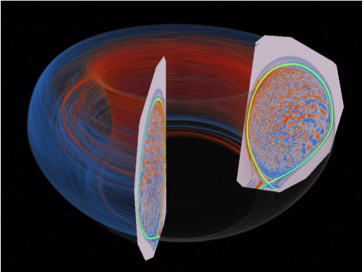
\includegraphics[width=.5\textwidth]{figures/xgcTokamakSimulation.png} \\
        \small{3D tokamak simulation.  2 poloidal planes shown.}
        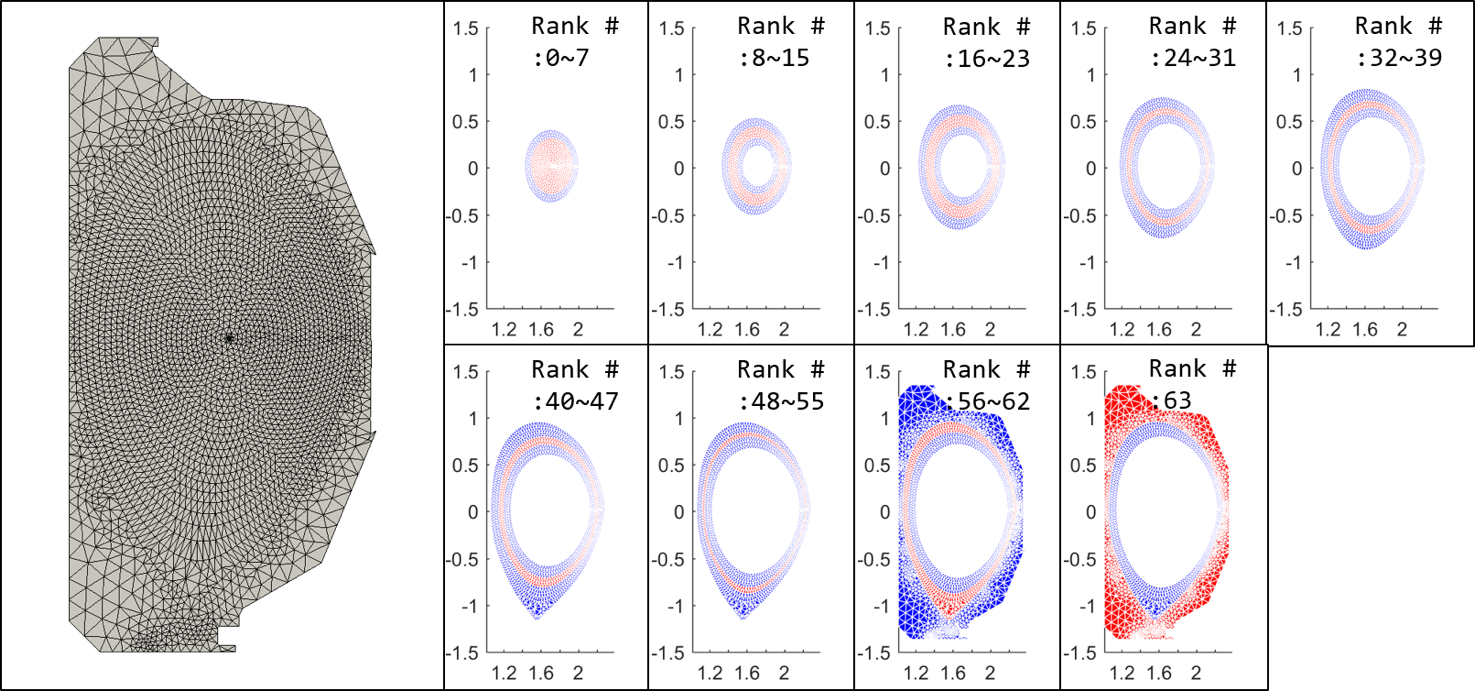
\includegraphics[width=.85\textwidth]{figures/xgcMeshDistribution.png} \\
        \small{2D mesh and process groups.}
      \end{figure}
    \end{column}
  \end{columns}
\end{frame}

\begin{frame}
  \frametitle{XGC - Early Summit Results (CS Chang)}
  \begin{columns}
    \begin{column}{0.5\textwidth}
      Strong Scaling vs Titan
      \begin{itemize}
        \item Scaling runs using up to 44\% of Summit, 2048 nodes
        \item MPI + CUDA (electron push) + OpenACC (collision) + OpenMP
        \item 25 times faster than Titan % HERE
      \end{itemize}
      CPU+GPU performance is 11 times faster than CPU only at 12,288 GPUs (2Ki
      nodes)
    \end{column}
    \begin{column}{0.5\textwidth}
      \begin{figure}
        \centering
        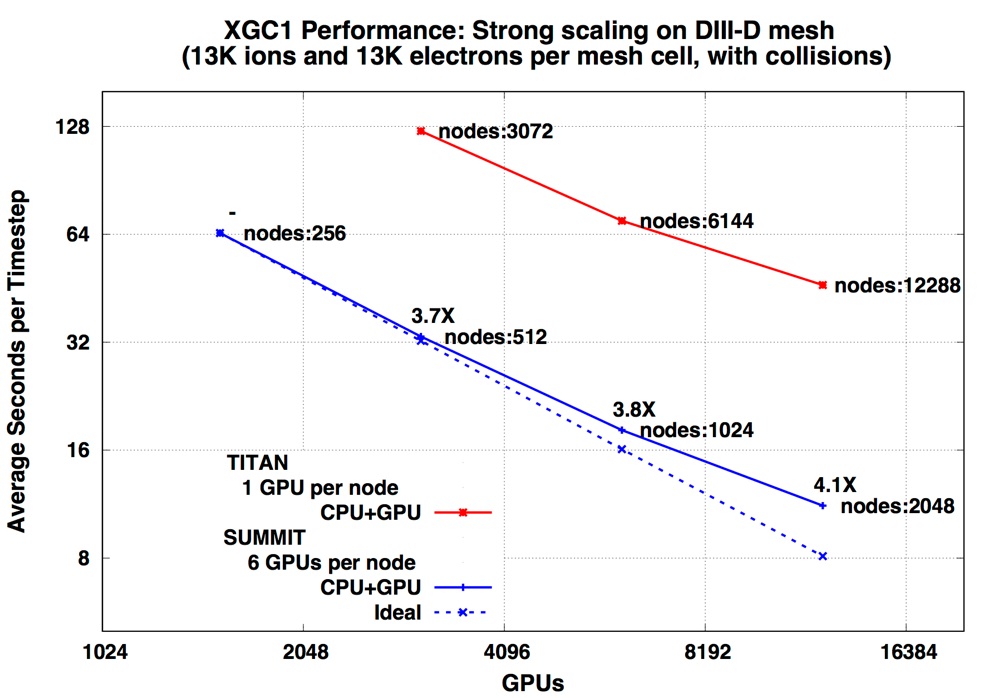
\includegraphics[width=\textwidth]{figures/xgcStrongScaling.png}
      \end{figure}
    \end{column}
  \end{columns}
\end{frame}

\begin{frame}
  \frametitle{XGC - Ongoing Developments}
  \begin{columns}
    \begin{column}{0.5\textwidth}
      Developing tools for unstructured mesh PIC
      \begin{itemize}
        \item Extending ECP COPA Cabana (Kokkos) - per element particle grouping 
          inspired by Sell-C-$\sigma$ rotated and padded CSR-like structure
        \item Distributed mesh with `safe' zones to avoid communication during
          push
        \item Bulk communication protocol that accounts for `safe' zones
        \item Particle load balancing with EnGPar
      \end{itemize}
    \end{column}
    \begin{column}{0.5\textwidth}
      \begin{figure}
        \centering
        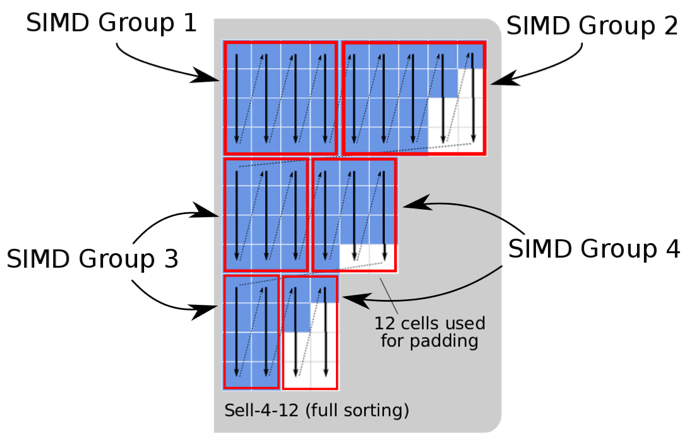
\includegraphics[width=.6\textwidth]{figures/sellCSigma.png}\\
        \small{Sell-C-$\sigma$ data structure.} \smallskip \\
        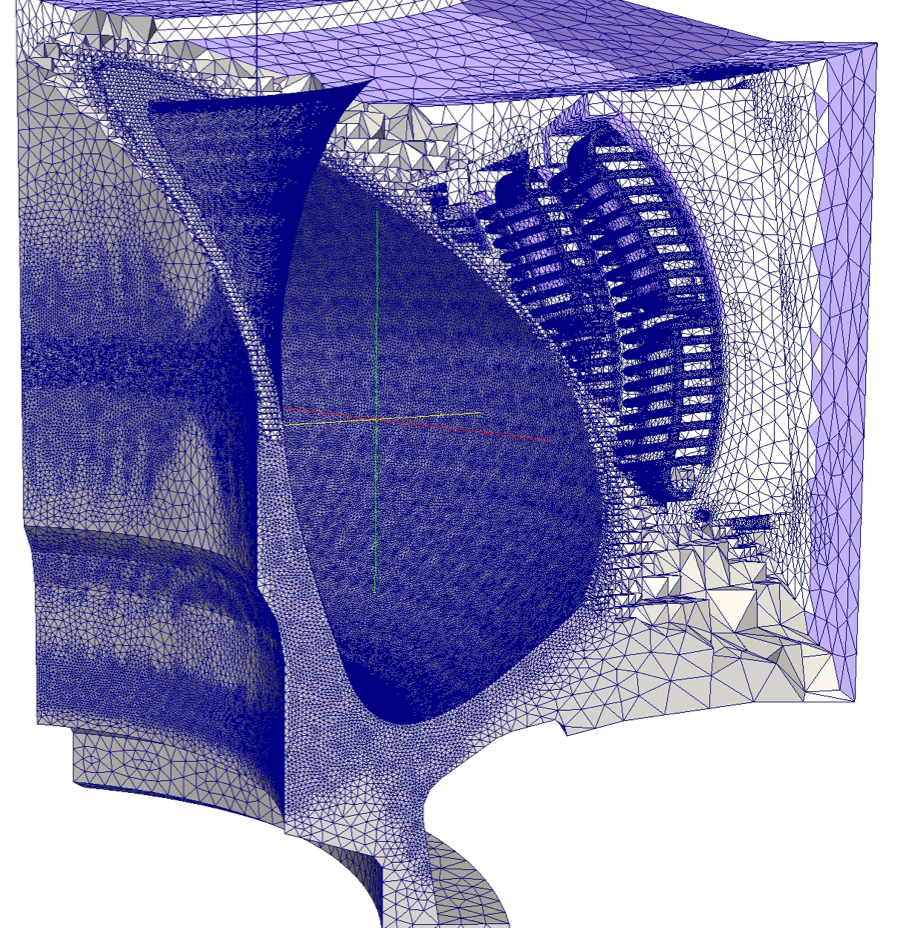
\includegraphics[width=.4\textwidth]{figures/rfMesh.png}\\
        \small{Unstructured 3D mesh of RF model.}
      \end{figure}
    \end{column}
  \end{columns}
\end{frame}

\begin{frame}
  \frametitle{MFEM Laghos MiniApp - High-order Compressible Gas Dynamics}
  Tzanio Kolev and Vladimir Tomov, Lawrence Livermore National Laboratory \\
  DOE Exascale Computing Project: The Center for Efficient Exascale Discretizations (CEED)
  \begin{columns}
    \begin{column}{0.5\textwidth}
      Goals
      \begin{itemize}
	\item Help applications leverage future architectures by providing them high
          order unstructured mesh methods.
        \item Collaborate with hardware vendors and software projects to guide
          the design of upcoming exascale systems.
      \end{itemize}
    \end{column}
    \begin{column}{0.5\textwidth}
      \begin{figure}
        \centering
        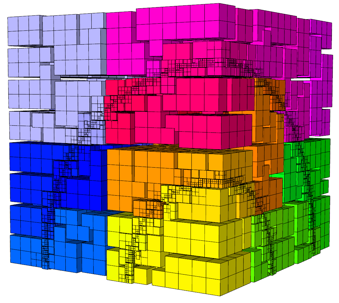
\includegraphics[width=.7\textwidth]{figures/laghos_sedov.png} \\
        \tiny{The Laghos miniapp's Sedov blast wave problem.  Laghos solves the
        time-dependent Euler equation of compressible gas dynamics in a moving
        Lagrangian frame using high-order finite element spatial discretization
        and explicit high-order time-stepping.}
      \end{figure}
    \end{column}
  \end{columns}
\end{frame}

\begin{frame}
  \frametitle{MFEM Laghos MiniApp - Partitioning Approach (T. Kolev, V. Tomov)}
  \begin{columns}
    \begin{column}{0.5\textwidth}
      \begin{itemize}
	\item One MPI process per GPU
        \item Initial partition with METIS
        \item Non-conforming adaptive mesh refinement (AMR) version using space
          filling curves
        \item GPU porting of computationally dominant functions in AMR version is underway
      \end{itemize}
    \end{column}
    \begin{column}{0.5\textwidth}
      \centering
      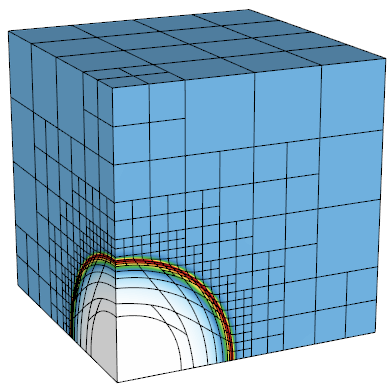
\includegraphics[width=0.3\textwidth]{figures/sedov-amr-900.png}
      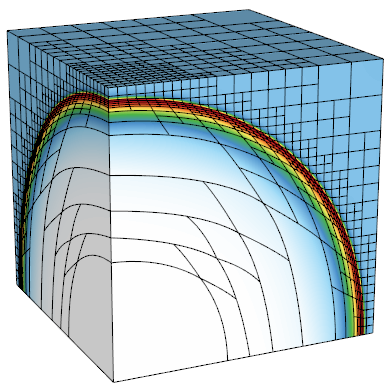
\includegraphics[width=0.3\textwidth]{figures/sedov-amr-2463.png} \\
      \small{Sedov AMR at steps 900 and 2463.} \\
      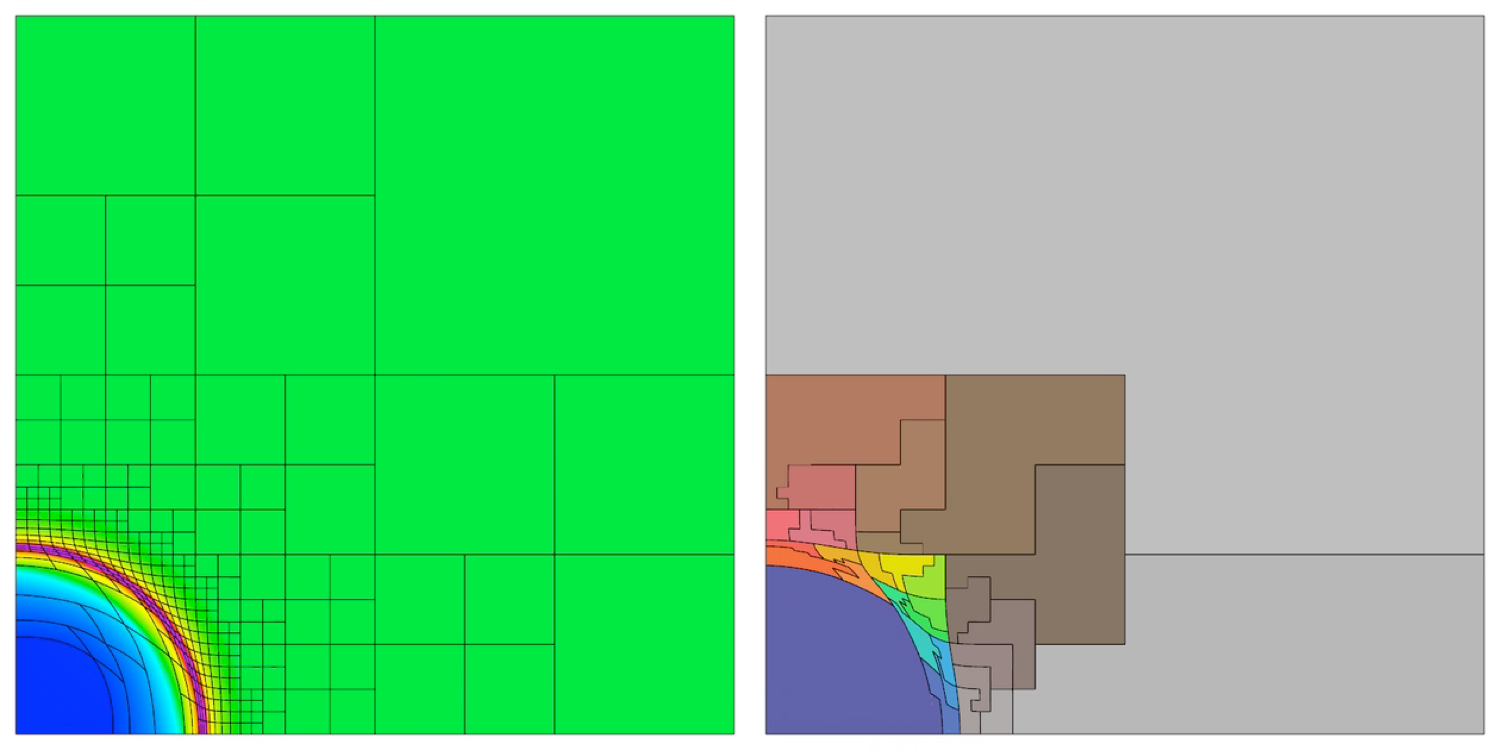
\includegraphics[width=0.9\textwidth]{{figures/sedov_animation_t8.19}.jpg} \\
      \small{Sedov AMR mesh (left) and partition (right) with space filling curves.}
    \end{column}
  \end{columns}
\end{frame}

\begin{frame}
  \frametitle{MFEM Laghos MiniApp - Early Sierra Results (T. Kolev, V. Tomov)}
  \begin{columns}
    \begin{column}{0.5\textwidth}
      \begin{itemize}
        \item 3rd order velocity and position (continuous kinematic), 2nd order internal
          energy (discontinuous thermodynamic) finite elements (Q3Q2)
        \item Mesh vertex repositioning without AMR
        \item Four GPUs/node with one MPI process/GPU
        \item More than 256K elements ('zones') required for
          scaling to ~30 GPUs, 16M elements required for 1024 GPUs
      \end{itemize}
    \end{column}
    \begin{column}{0.5\textwidth}
      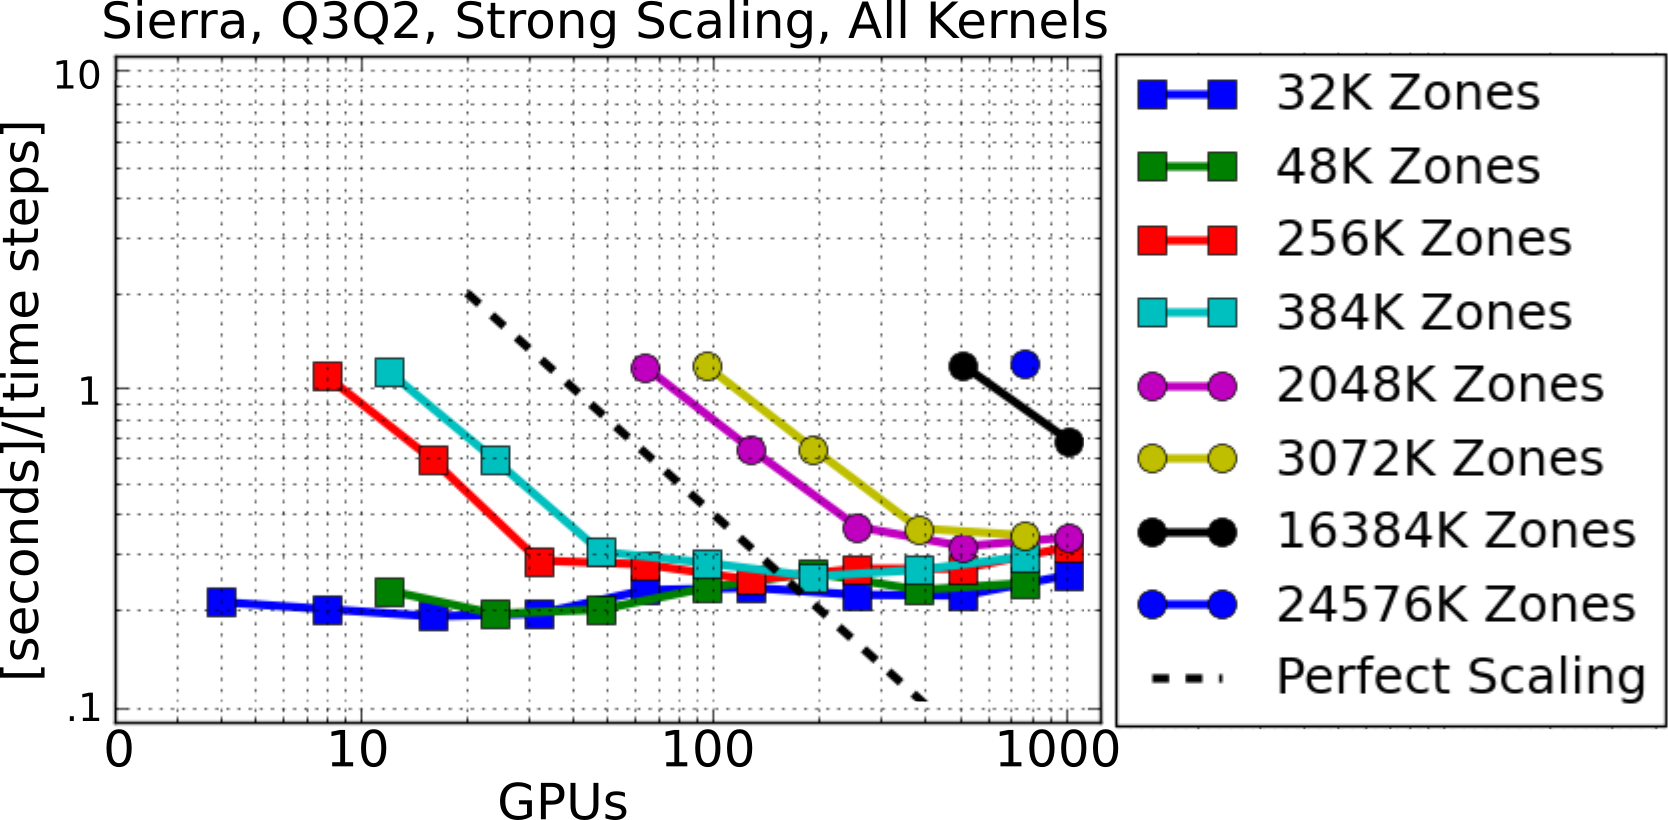
\includegraphics[width=\textwidth]{figures/laghos_strong_Q3Q2_sierra_cws.png} \\
      \small{Strong scaling for Laghos on Sierra of pure CUDA version.
      A zone is a mesh element.}
    \end{column}
  \end{columns}
\end{frame}

\begin{frame}

  \frametitle{MFEM Laghos MiniApp - Next Steps for Load Balancing AMR}
  Task Mapping
  \begin{itemize}
    \item Ensure proceses that are assigned to the same node share domain data
    \item Zoltan2 (Karen Devine, SNL) geometric methods support the mapping of
      the network partition to the domain partition
  \end{itemize}
  SFC
  \begin{itemize}
    \item Implement on-node balancer to avoid inter-node communications
    \item As needed, run global balancer when execution cost on
      imbalanced mesh is factors more than the cost to fix the imbalance
  \end{itemize}
  EnGPar
  \begin{itemize}
    \item Integrate EnGPar w/MFEM - similar interface as (Par)METIS
    \item Complete acceleration of critical EnGPar procedures - initial work
      completed with Kokkos
  \end{itemize}
\end{frame}

\begin{frame}
  \frametitle{Closing Remarks and Future Work}
  MPI tests show that EnGPar:
  \begin{itemize}
    \item Quickly reduces the high secondary imbalances on up to 512Ki parts
    \item Maintains edge cut and primary imbalances
  \end{itemize}
  Inter-GPU data movement is expensive. Some possible mitigations:
  \begin{itemize}
    \item placing processes near those they share domain data with
    \item balancing within each node before addressing inter-node imbalance
    \item optimizing partitions for communication, possibly sacrificing load imbalance
    \item buffering and compressing messages
    \item overlapping communication with computation
    \item predictively load balancing
    \item ghosting mesh in host memory
  \end{itemize}
\end{frame}

\begin{frame}
  \begin{center}
    {\huge
      Thank You\\
      \bigskip
      \bigskip
      \bigskip
      \bigskip
      \bigskip
      \huge
      Questions?\\
      \bigskip
      \bigskip
      \bigskip
    }
  \end{center}
  \large
  Acknowledgements:\\
  \begin{itemize}
    \item NSF SI2-SSE: Fast Dynamic Load Balancing Tools for Extreme Scale Systems
    \item DOE FASTMath SCIDAC Institute
    \item CEED ECP
  \end{itemize}
\end{frame}

\end{document}
